\documentclass[10pt]{article}
\usepackage[utf8]{inputenc}
\usepackage[dvips]{graphicx}
\usepackage{fancybox}
\usepackage{verbatim}
\usepackage{array}
\usepackage{latexsym}
\usepackage{alltt}
\usepackage{hyperref}
\usepackage{textcomp}
\usepackage{color}
\usepackage{amsmath}
\usepackage{amsfonts}
\usepackage{tikz}
\usepackage{fitch}  % to use fitch
\usepackage{float}
\usepackage[hmargin=3cm,vmargin=5.0cm]{geometry}
%\topmargin=0cm
\topmargin=-2cm
\addtolength{\textheight}{6.5cm}
\addtolength{\textwidth}{2.0cm}
%\setlength{\leftmargin}{-5cm}
\setlength{\oddsidemargin}{0.0cm}
\setlength{\evensidemargin}{0.0cm}


\begin{document}

\section*{Student Information } 
%Write your full name and id number between the colon and newline
%Put one empty space character after colon and before newline
Full Name :  Emre Geçit\\
Id Number :  2521581\\


% ND example using fitch
% delete or comment if you intend to use this to generate the vector pdf 
\section*{Q. 1}
$(A \cup B)\symbol{92}(A \cap B)=\big\{x|x\in (A \cup B) \land \neg x\in (A \cap B) \big\}$ Definition of difference \\
$=\big\{x|x\in (A \cup B) \land \neg((x \in A) \land (x \in B)) \big\}$ Definition of intersection \\
$=\big\{x|x\in (A \cup B) \land (\neg(x \in A) \lor \neg(x \in B)) \big\}$ De Morgan's rule for logical operations \\
$=\big\{x|((x\in (A \cup B)) \land \neg(x \in A)) \lor (x \in (A \cup B)\land \neg(x \in B)) \big\}$ Distributive law \\
$=\big\{x|((x\in A \lor x\in B) \land \neg(x \in A)) \lor ((x \in A \lor x \in B)\land \neg(x \in B)) \big\}$ Definition of union \\
$=\big\{((x \in A \land \neg (x \in A)) \lor (x \in B \land \neg (x \in A))) \lor ((x \in A \land \neg (x \in B)) \lor (x \in B \land \neg (x \in B))) \big\}$ Distributive law \\
$=\big\{((F \lor (x \in B \land \neg (x \in A))) \lor ((x \in A \land \neg (x \in B)) \lor F)\big\}$ Complement law \\
$=\big\{(x \in B \land \neg (x \in A)) \lor (x \in A \land \neg (x \in B))\big\}$ Domination law \\
$=\big\{(x \in A \land \neg (x \in B)) \lor (x \in B \land \neg (x \in A)\big\}$ Commutative law \\
$=\big\{(x \in A \symbol{92} B) \lor (x \in B \symbol{92} A)\big\}$ Definition of difference \\
$=\big\{x \in ((A \symbol{92} B) \cup (B \symbol{92} A))\big\}$ Definition of union \\

Conclusion:
$(A \cup B)\symbol{92}(A \cap B)=(A \symbol{92} B) \cup (B \symbol{92} A)$

\section*{Q. 2}
$\big\{f|f\subseteq\mathbb{N}\times{0,1}\big\}\symbol{92} \big\{f|f:\big\{0,1\big\}\rightarrow\mathbb{N}$, f is a function$\big\}\\\\
\big\{f|f\subseteq\mathbb{N}\times{0,1}\big\}=P(N\times{0,1})$\\
$|\mathbb{N}\times \big\{0, 1\big\}| = 2|\mathbb{N}|$\\
Since $|\mathbb{N}|$ is countably infinite, 2$|\mathbb{N}|$ is countably infinite as well.\\
Power set of a countably infinite set is an uncountable set.
So, the left-hand side of the difference is an uncountable set.\\
Proof that the right-hand side is a countable set:\\

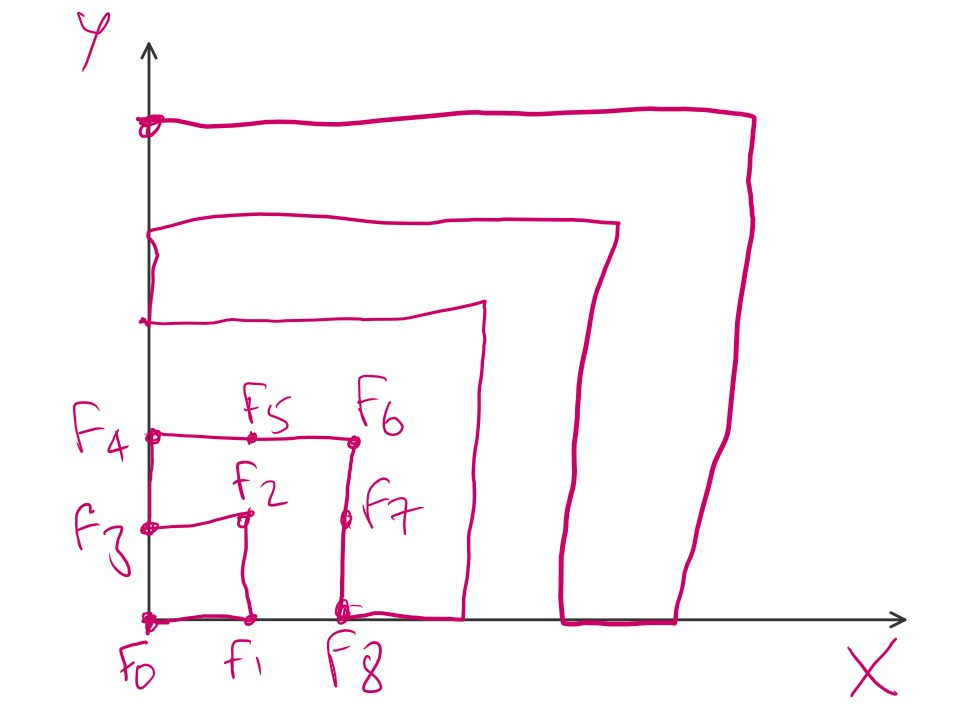
\includegraphics[scale=0.2]{proof.jpeg}\\
In this graph, every point represents a function, and for any function on this graph, the x value corresponds to the f(0) value, and the y value corresponds to the f(1) value. Since the curve passes over all the natural number to natural number combinations, with that enumeration method, all the functions in the set can be enumerated.\\
In the LHS of the difference there is a uncountable set, in the RHS, there is a countable set.\\\\
Proof that UNCOUNTABLE$\symbol{92}$COUNTABLE is uncountable:\\
Let A be an uncountable set, B be a countable set.\\
$B\cup(A\symbol{92}B) = B\cup(A\cap\overline{B})$ By the definition\\
$=(B\cup A)\cap(B\cup \overline{B})$ Distributive law\\
$=(B\cup A)\cap U$ Complement law\\
$=B\cup A$ Domination law\\
Conclusion: $B\cup(A\symbol{92}B)=B\cup A$\\
$B\cup A$ is an uncountable set since A is uncountable.\\
Then,  $B\cup(A\symbol{92}B)$ is uncountable.\\
Since B is countable, $(A\symbol{92}B)$ must be uncountable in order $B\cup(A\symbol{92}B)$ to be uncountable.\\
Conclusion: UNCOUNTABLE$\symbol{92}$COUNTABLE is uncountable\\\\
Since the left-hand side of the difference is uncountable and the right-hand side of the difference is countable, and UNCOUNTABLE$\symbol{92}$COUNTABLE is uncountable, the whole expression is uncountable.


\section*{Q. 3}
Assume that $4^n+5n^2log(n)=O(2^n)\\
c.2^n\geq 4^n+5n^2log(n) \quad \exists k \exists c \forall n, n\geq k$ (Definition of big O)\\
$c.2^n \geq 4^n \quad \exists k \exists c \forall n, n\geq k\\
c.2^n \geq 2^{2n} \quad \exists k \exists c \forall n, n\geq k\\
c \geq 2^{n} \quad \exists k \exists c \forall n, n\geq k \quad (2^n>0)$\\
Since $2^n$ goes to infinite as n goes to infinite, there cannot be such c. In other words, no matter how, big c is, there will always be some n$\geq$k such that $2^n>$c. Since we reached a contradiction, we can conclude that our assumption is false.\\\\
Conclusion: $4^n+5n^2$ is not $O(2^n)$
\section*{Q. 4}
$(2x-1)^n-x^2\equiv -x-1 (mod(x-1))$\\
$(2x-1)^n\equiv -x-1+x^2 (mod(x-1))$\\
$(2x-1)^n mod(x-1) = (-x-1+x^2)mod(x-1)$\\
$(2x-1)^n mod(x-1) = ((x-1).(x-1)+x-2) mod(x-1)$\\
((x-1).(x-1)+x-2)mod(x-1) = x-2 (Since x$>$2, the result is guaranteed to be positive. Moreover, since x-2 $<$ x-1, the remainder is smaller than the divider and no rule is violated)\\
$(2x-1)^n mod(x-1) = ((2x-1)mod(x-1))^n$\\
$2x-1 = 2(x-1) + 1 \rightarrow (2x-1)^n mod(x-1) = 1$\\
$(2x-1)^n mod(x-1) = 1^n = 1\\$
$1 = x-2\\
x = 3$
\end{document}